\documentclass[jou]{apa6}
\usepackage[utf8]{inputenc}
\usepackage[spanish]{babel}

\usepackage{csquotes}
\usepackage[style=apa,sortcites=true,sorting=nyt,backend=biber]{biblatex}

\usepackage{listings}

\usepackage[section]{placeins}

\DeclareLanguageMapping{spanish}{spanish-apa}
\addbibresource{bibliography.bib}

\title{HPC - LAB3: Paradigma SIMT - CUDA}

\author{Rubén Cavieres Carvajal}
\affiliation{Universidad de Santiago de Chile}

\leftheader{DIINF-USACH}

\shorttitle{HPC - LAB3}

\abstract{Se presenta un resumen del desarrollo del laboratorio 3 de la asignatura High Performance Computing dictado por el profesor Dr. Fernando Rannou, exponiendo resultados de las pruebas de rendimiento computacional sobre la aplicación paralelizada.}

\keywords{HPC, CUDA, NVIDIA, Parallel, Schroedinger}

\begin{document}
\maketitle
El trabajo comienza con la creación de un algoritmo secuencial que simula el comportamiento de una onda bajo la ley de Schroedinger.

Luego se identifican las piezas de código que pueden ser paralelizables para utilizar en estas estrategias basadas en el paradigma SIMT-CUDA.

Finalmente se realizan pruebas de rendimiento de la aplicación utilizando las métricas:

\begin{itemize}
	\item Tiempo de ejecución (wall-clock) para diferentes tamaños de grillas.
	\item Ocupancia
	\item Tiempo de ejecución para diferentes tamaños de bloques.
\end{itemize}


\section{Algoritmo}
\subsection{Ecuaciones}
El algoritmo se estructuró de tal forma que represente el planteamiento del matemático. Es decir, consideró las condiciones de la variable tiempo $t$ para utilizar las ecuaciones con los siguientes métodos:

\begin{itemize}
	\item \texttt{initializeSpace}: Para $t = 0$ inicializa el espacio (grilla) de trabajo, dado por el impulso en celdas centrales en grilla.
	\item \texttt{fillSpaceFirstStep}: Para $t = 1$ genera la primera iteración de la onda utilizando $H^{t-1}$.
	\item \texttt{fillSpaceTSteps}: Para $t > 1$ genera las sucesivas iteraciones de la onda, utilizando los estados del espacio $H^{t-1}$ y $H^{t-2}$.
\end{itemize}

\subsection{Paralelización}
La estrategia de paralelización se basó en descubrir los bloques de códigos críticos potenciales para la utilización de CUDA.

Estos trozos de código son aquellos que construyen la ecuación de Schroedinger para el intervalo de tiempo $t >= 1$ (método \texttt{fillSpaceTSteps}):

\lstset{language=C, breaklines=true, frame=single}

\begin{lstlisting}
int i = blockIdx.y * blockDim.y + threadIdx.y;
int j = blockIdx.x * blockDim.x + threadIdx.x;

waveSpace[N * i + j] = 2 * waveSpaceTMin1[N * i + j] - waveSpaceTMin2[N * i + j] + (c * c) * (dt/dd * dt/dd) * (waveSpaceTMin1[N * (i + 1) + j] + waveSpaceTMin1[N * (i - 1) + j] + waveSpaceTMin1[N * i + (j - 1)] + waveSpaceTMin1[N * i + (j + 1)] - 4 * waveSpaceTMin1[N * i + j]);
\end{lstlisting}

La estrategia adoptada fue la de utilizar las posiciones absolutas de las hebras dentro de la grilla completa, para así procesar cada porción del arreglo que contendrá imagen con expansión de onda a generar.

De esta manera, se obtienen los indices \texttt{i, j} a partir del identificador de bloque, tamaño de éste y la identificación de hebra actual.

Las matrices necesarias para operar la ecuación son entregadas por parámetro a la función, utilizando memoria compartida. Cada vez que termina de ejecutarse el método, se reasignan los valores de las matrices a sus nuevos estados \texttt{T}:

\lstset{language=C, breaklines=true, frame=single}

\begin{lstlisting}
cudaMemcpy(waveSpaceTMin2_d, waveSpaceTMin1_d, N * N * sizeof(float), cudaMemcpyDeviceToDevice);
cudaMemcpy(waveSpaceTMin1_d, waveSpace_d, N * N * sizeof(float), cudaMemcpyDeviceToDevice);
\end{lstlisting}

Cada copia de esta información se concentra en dispositivo.

\section{Rendimiento Computacional}

El análisis de rendimiento se realizó bajo los siguientes parámetros y tamaños:

\begin{itemize}
	\item Grillas = \{512, 1024, 2048, 4096\}
	\item Bloques = \{10x10, 16x16, 32x16, 32x32\}
	\item Tiempo = \{300, 1000, 10000\}
\end{itemize}

En un principio se ejecutaron las pruebas con el algoritmo generando imagen en formato RAW, pero por problemas de capacidad de almacenamiento de equipos computacionales y lentitud de ejecución, debió modificarse el algortimo para evitar la generación de las imágenes para cada caso.

A pesar de lo anterior se lograron ejecutar pruebas con algoritmo original (generando imagen) hasta la iteración \texttt{N = 4096, T = 300}, cuyas pruebas son expuestas en apartado.

\subsection{Tiempo (Mismo Tamaño de Bloque)}

Para los siguientes cálculos se utilizaron como tamaño de bloque \texttt{X = 10, Y = 10}:

\begin{itemize}
	\item Con generación de la imagen de salida
	\item Sin generación de la imagen de salida.
\end{itemize}

\subsubsection{Sin Generación Imagen Salida}
El tiempo tomado para realizar la ejecución se representa en la siguiente figura:

\begin{figure}[h]
	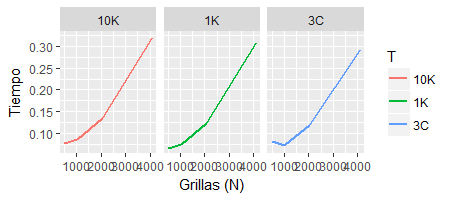
\includegraphics[width=\columnwidth]{time-same-block-size-no-raw.png}
	\caption{Tiempo ejecución para T = \{300, 1000, 10000\}}
	\label{fig:Figure1}
\end{figure}

En los tres casos el tiempo aumenta aceleradamente en una proporción similar como se evidencia en curvas. 

Sin embargo, se destaca que al aumentar el número de pasos \texttt{T}, el rendimiento del procesamiento siga siendo similar, demostrando la capacidad de la unidad GPU de procesar tareas de cómputo repetitivas. 

Se obtienen los siguientes mínimos: 

% Please add the following required packages to your document preamble:
% \usepackage{booktabs}
\begin{table}[h]
\centering
\caption{Mínimos de tiempo por iteraciones.}
\label{my-label}
\begin{tabular}{@{}lll@{}}
\toprule
\multicolumn{1}{c}{T (its.)} & \multicolumn{1}{c}{N (grilla.)} & \multicolumn{1}{c}{T (seg.)} \\ \midrule
300                          & 1024                         & 0,073585                     \\
1000                         & 512                          & 0,066303                     \\
10000                        & 512                          & 0,076833                     \\ \bottomrule
\end{tabular}
\end{table}

Como se ha dicho, estos mínimos se incrementan aceleradamente a medida que aumentan las iteraciones.

\FloatBarrier

\subsubsection{Con Generación Imagen Salida}
Ejecutando algoritmo con generación de imagen, se consigue siguiente rendimiento:

\begin{figure}[h]
	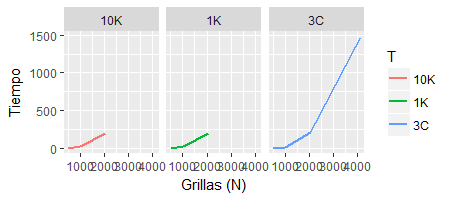
\includegraphics[width=\columnwidth]{time-same-block-size-with-raw.png}
	\caption{Tiempo ejecución para T = \{2000, 4000, 8000\}}
	\label{fig:Figure2}
\end{figure}

No fue posible continuar con resto de pruebas, debido al llenado de espacio en disco duro de computador, producto de la imagen de gran tamaño que se estaba generando para \texttt{N = 4096, T = 1000}.

El comportamiento de la curva en comparación al anterior es equivalente, registrando los siguientes mínimos:

\begin{table}[h]
\centering
\caption{Mínimos de tiempo por iteraciones.}
\label{my-label}
\begin{tabular}{@{}lll@{}}
\toprule
\multicolumn{1}{c}{T (its.)} & \multicolumn{1}{c}{N (grilla.)} & \multicolumn{1}{c}{T (seg.)} \\ \midrule
300                          & 512                          & 0.244316                     \\
1000                         & 512                          & 0.284443                     \\
10000                        & 512                          & 0.296664                     \\ \bottomrule
\end{tabular}
\end{table}

\clearpage

Los tiempos mínimos no experimentan mayores cambios, en comparación con los máximos:

\begin{table}[h]
	\centering
	\caption{Máximos de tiempo por iteraciones.}
	\label{my-label}
	\begin{tabular}{@{}lll@{}}
		\toprule
		\multicolumn{1}{c}{T (its.)} & \multicolumn{1}{c}{N (grilla.)} & \multicolumn{1}{c}{T (seg.)} \\ \midrule
		300                          & 4096                         & 25 (min)                     \\
		1000                         & 2048                         & 3,4 (min)                    \\
		10000                        & 2048                         & 3,4 (min)                    \\ \bottomrule
	\end{tabular}
\end{table}

Dichos tiempos fueron excesivamente altos comparándolos a su ejecución sin almacenamiento de imagen, evidenciando el costo computacional que implica el acceso a memoria secundaria, por ser aquella más lenta dentro de todos los tipos de memoria del sistema.

\FloatBarrier

\subsection{Ocupancia}
La métrica utilizada para calcular el \textit{Device Occupancy} se expresa de la siguiente forma:

\[
	Ocupancia = \frac{Numero\, de\, warps\, activos}{Maximo\, Numero\, de\, warps}
\]

Para dicha labor se utilizó la herramienta \textit{CUDA Occupancy calculator}, que permite realizar el calcular la ocupancia de un kernel particular a partir de las siguientes entradas:

\begin{itemize}
	\item Compute capability = 5,2 (A partir de información recogida para GPU NVIDIA Quadro M2000)
	\item Shared memory size Config (bytes) = 98304
	\item Global load caching mode = L2 only (cg)
	\item Threads per block = 1024 (considerando el tamaño máximo de bloques utilizado)
	\item Registers per thread = 18 (a partir de comando \texttt{nvcc --ptxas-options=-v})
	\item Shared memory per block (bytes) = 88
\end{itemize}



Consiguendo la siguiente información:

% Please add the following required packages to your document preamble:
% \usepackage{booktabs}
\begin{table}[h]
	\centering
	\caption{Ocupancia GPU}
	\label{my-label}
	\begin{tabular}{@{}ll@{}}
		\toprule
		Active Threads per Multiprocessor         & 2048           \\ \midrule
		Active Warps per Multiprocessor           & 64             \\
		Active Thread Blocks per Multiprocessor   & 2              \\
		\textbf{Occupancy of each Multiprocessor} & \textbf{100\%} \\ \bottomrule
	\end{tabular}
\end{table}

Se alcanza máxima ocupancia con la solución construída.

\subsection{Tiempo (Diferentes Tamaños de Bloques, Sin Imagen Salida)}
Para este caso se utilizaron los parámetros:

\begin{itemize}
	\item Grilla = \{2048x2048\}
	\item Bloques = \{16x16, 32x16, 32x32\}
	\item Tiempo = \{300, 1000, 10000\}
\end{itemize}

Curva generada fue la siguiente:

\begin{figure}[h]
	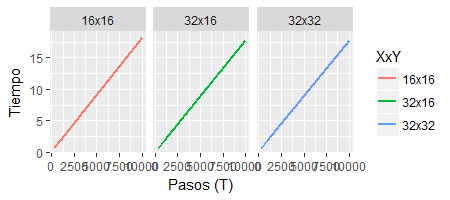
\includegraphics[width=\columnwidth]{time-diff-block-size-no-raw.png}
	\caption{Tiempo ejecución para T = \{300, 1000, 10000\}}
	\label{fig:Figure3}
\end{figure}

Cambiando el tamaño de los bloques se aprecia un comportamiento lineal similar al aumentar el valor \texttt{T}.

\section{Conclusiones}

El trabajo mostró el desempeño la implementación de la ecuación de Schroedinger, bajo el paradigma CUDA-SIMT.

Los gráficos generados muestran un comportamiento uniforme del desempeño para cada caso comparado, siendo en términos generales consistente la ejecución del algoritmo ante el aumento de carga y utilización de tamaños de bloques distintos.

Un problema experimentado en el análisis fue la ejecución de las pruebas con algoritmo generado imagen extensión RAW, que ante una iteración con valores altos, consumió tiempo y espacio en disco duro excesivo, obligando a quitar esta opción para continuar con análisis, descubriendo un considerable incremento en el rendimiento de la aplicación.

\end{document}
